
\chapter*{Results}
\label{sec:orgdc906dd}

\section*{Impact of mapping in the overall circuit error}
\label{sec:orga4d162e}

\begin{table}[htbp]
\caption{Table of the selected benchmarks to be mapped. Note that the crossed ones mean that they were to}
\centering
\small
\begin{tabular}{llll}
\hline
Benchmark & \# qubits & \# gates & two-qubit gates (\%)\\
\hline
sf\(_{\text{274}}\) & 6 & 781 & 0.430\\
mod5adder\(_{\text{127}}\) & 6 & 555 & 0.431\\
sf\(_{\text{276}}\) & 6 & 778 & 0.432\\
4gt4\(_{\text{v0}}\)\(_{\text{72}}\) & 6 & 258 & 0.438\\
decod24\(_{\text{bdd}}\)\(_{\text{294}}\) & 6 & 73 & 0.438\\
mod10\(_{\text{176}}\) & 5 & 178 & 0.438\\
sym6\(_{\text{145}}\) & 7 & 3888 & 0.438\\
4gt12\(_{\text{v1}}\)\(_{\text{89}}\) & 6 & 228 & 0.439\\
decod24\(_{\text{enable}}\)\(_{\text{126}}\) & 6 & 338 & 0.441\\
4mod5\(_{\text{bdd}}\)\(_{\text{287}}\) & 7 & 70 & 0.443\\
mod8\(_{\text{10}}\)\(_{\text{177}}\) & 6 & 440 & 0.445\\
one\(_{\text{two}}\)\(_{\text{three}}\)\(_{\text{v1}}\)\(_{\text{99}}\) & 5 & 132 & 0.447\\
alu\(_{\text{bdd}}\)\(_{\text{288}}\) & 7 & 84 & 0.452\\
one\(_{\text{two}}\)\(_{\text{three}}\)\(_{\text{v3}}\)\(_{\text{101}}\) & 5 & 70 & 0.457\\
hwb4\(_{\text{49}}\) & 5 & 233 & 0.459\\
rd32\(_{\text{v0}}\)\(_{\text{66}}\) & 4 & 34 & 0.471\\
alu\(_{\text{v0}}\)\(_{\text{27}}\) & 5 & 36 & 0.472\\
4mod5\(_{\text{v0}}\)\(_{\text{20}}\) & 5 & 20 & 0.500\\
ham3\(_{\text{102}}\) & 3 & 20 & 0.550\\
mod5d1\(_{\text{63}}\) & 5 & 22 & 0.591\\
4gt11\(_{\text{82}}\) & 5 & 27 & 0.667\\
xor5\(_{\text{254}}\) & 6 & 7 & 0.714\\
graycode6\(_{\text{47}}\) & 6 & 5 & 1.000\\
\hline
\end{tabular}
\end{table}

\label{tab:map_selected_benchs}
\begin{figure}[htbp]
\centering
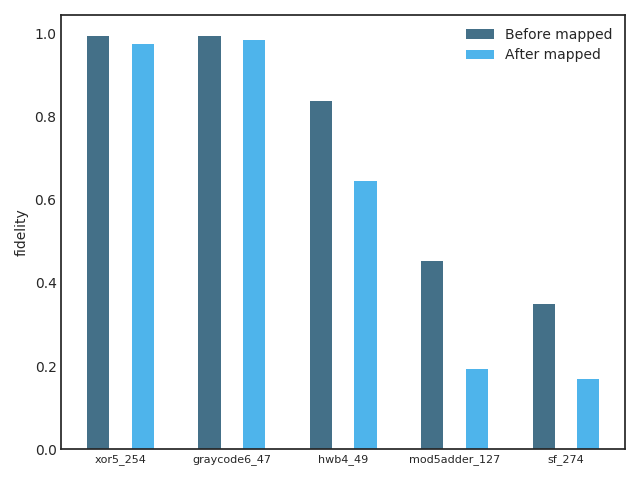
\includegraphics[width=\textwidth]{figures/f_diff_bar_plot.png}
\caption{\label{fig:orgdd3a509}
}
\end{figure}
\begin{figure}[htbp]
\centering
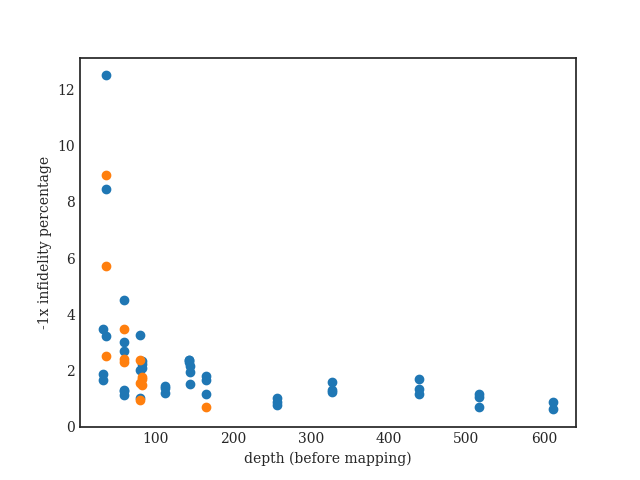
\includegraphics[width=\textwidth]{figures/infid_percentage_depth_before_mapping.png}
\caption{\label{fig:org9be5637}
}
\end{figure}


\subsection*{:noexport:}
\label{sec:orgd07399d}

\begin{itemize}
\item In order to get this figure we filter fidelity. Only f>0.5 is plot
\item Infidelity: \(\frac{f_a - f_b}{1 - f_b}\)
\item Depth is the depth before mapping
\item We decided to see it like this in order to cluster the same benchmark mapped in different ways
\item We can conclude that the mapper quality is critical for benchmarks with small depth before being mapped, but for long circuits the mapper quality gets diminished. This means that simple and, therefore, faster mappers can be implemented for long circuits making possible the mapping on the fly, for instance
\end{itemize}

\section*{Analysis of the mapping metrics}
\label{sec:orgd531432}

\begin{center}
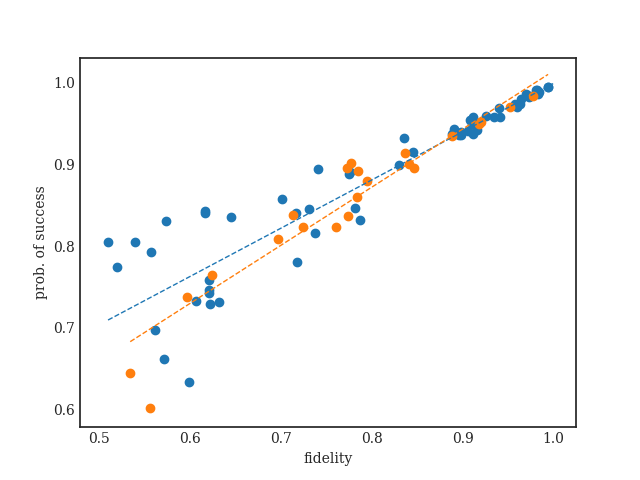
\includegraphics[width=.9\linewidth]{figures/f_ps_correlation_with_meas_error.png}
\end{center}

\begin{center}
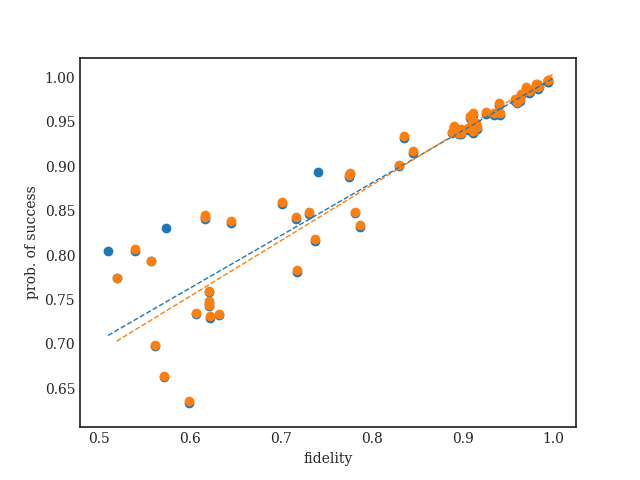
\includegraphics[width=.9\linewidth]{figures/f_ps_correlation_no_meas_error.png}
\end{center}


\subsection*{Metrics behaviour}
\label{sec:orgb965b8d}




\begin{itemize}
\item :noexport:
\label{sec:org18e6dcf}

SIGO FILTRANDO FIDELITY > 0.5

\begin{minted}[frame=lines,fontsize=\scriptsize,linenos,breaklines,breakanywhere]{c}

	Analysis For Decoherence Time = 3000 and Error Measurement = 0.005

	-------------------------------

	-- Correlation between Fidelity and:

- # of Gates:

Polynomial function:
	   2
1.534e-07 x - 0.000523 x + 1.005
----------------------------

(-0.8630740403512944, 7.492413733912921e-19)

- # of two-qubit gates:

Polynomial function:
	   2
3.049e-06 x - 0.002383 x + 1.004
----------------------------

(-0.863286950097695, 7.18389012251959e-19)

- Depth:

Polynomial function:
	   2
3.203e-07 x - 0.0007814 x + 1.019
----------------------------

(-0.8305711564938272, 2.2460770328365885e-16)

- Quantum Volume:

Polynomial function:
	   2
4.242e-09 x - 8.926e-05 x + 0.9828
----------------------------

(-0.7902264007122082, 6.045814411414274e-14)


	-- Correlation between Probability of Success and:

- # of Gates:

Polynomial function:
	   2
1.425e-07 x - 0.0003704 x + 1.008
----------------------------

(-0.6324404022306189, 5.9408960728175597e-08)

- # of two-qubit gates:

Polynomial function:
	   2
2.769e-06 x - 0.001732 x + 1.01
----------------------------

(-0.6441233355408925, 2.8150298712169916e-08)

- Depth:

Polynomial function:
	   2
2.584e-07 x - 0.0005238 x + 1.014
----------------------------

(-0.6174470539858588, 1.4818911589874065e-07)

- Quantum Volume:

Polynomial function:
	   2
3.169e-09 x - 5.64e-05 x + 0.988
----------------------------

(-0.5724133147384978, 1.7659969011385104e-06)

	Analysis For Decoherence Time = 1000 and Error Measurement = 0.005

	-------------------------------

	-- Correlation between Fidelity and:

- # of Gates:

Polynomial function:
	   2
5.383e-07 x - 0.001103 x + 0.9934
----------------------------

(-0.897561920337874, 1.4957448590931355e-08)

- # of two-qubit gates:

Polynomial function:
	  2
1.629e-05 x - 0.005348 x + 0.9712
----------------------------

(-0.7785748517752366, 1.975273755557373e-05)

- Depth:

Polynomial function:
	   2
1.651e-06 x - 0.001773 x + 1.009
----------------------------

(-0.8194633195943474, 3.078535631273159e-06)

- Quantum Volume:

Polynomial function:
	   2
2.687e-08 x - 0.000201 x + 0.9471
----------------------------

(-0.6784205747012305, 0.0005194496207515033)


	-- Correlation between Probability of Success and:

- # of Gates:

Polynomial function:
	  2
2.03e-08 x - 0.0006141 x + 0.9941
----------------------------

(-0.8447301986384201, 7.618304513439932e-07)

- # of two-qubit gates:

Polynomial function:
	   2
3.226e-06 x - 0.002616 x + 0.9647
----------------------------

(-0.6901152561603443, 0.00037894800783273185)

- Depth:

Polynomial function:
	   2
6.506e-07 x - 0.001068 x + 1.009
----------------------------

(-0.792713984206436, 1.0880694258391198e-05)

- Quantum Volume:

Polynomial function:
	   2
1.125e-08 x - 0.0001186 x + 0.9648
----------------------------

(-0.6477821957243156, 0.0011155566982108602)


\end{minted}
\end{itemize}

\section*{Advice}
\label{sec:org62947ed}
